%!TEX root = ../../../adrien_gomar_phd.tex

\paragraph{Steady results}

For the subsonic case, 
the experimental inlet Mach number is $0.31$ 
and the isentropic outlet Mach number is $0.69$.
% steady results
Steady results for the isentropic Mach number at 
blade walls are compared to the experimental data in 
Figure~\ref{fig:stcf11_rans_subsonic}.  For this flow regime, the fluid
remains subsonic.
On the pressure side, the flow accelerates all the way
to the trailing edge of the blade. 
The stagnation point is located at $x / c \approx 0.05$.
On the suction side, 
the flow
accelerates until a maximum speed at $\approx 40~\%$ of the chord and
finally decelerates toward the trailing edge.
The agreement with the experimental data is fair. However, an
over-prediction of the isentropic Mach number is observed on the suction
side.  This discrepancy is also reported in the literature (see
\citet{Fransson1999} for instance).

\begin{figure}[htp]
  \centering
  \subfigure[isentropic Mach number at blade walls]{
  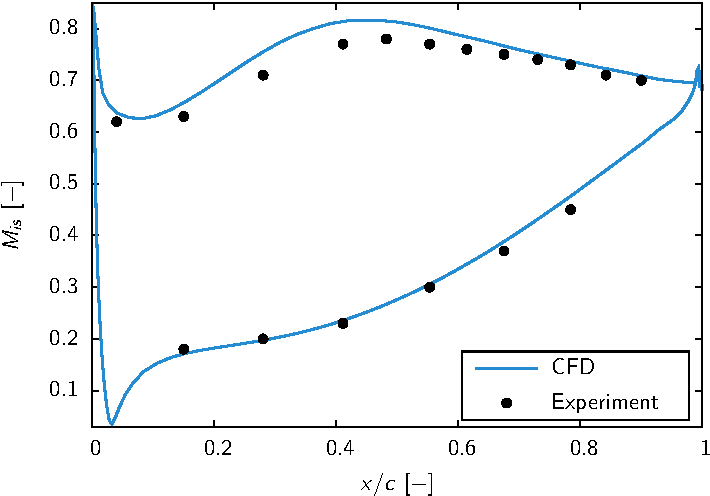
\includegraphics[height=.3\textwidth]{STCF11_RANS_SUBSONIC_PPT.pdf}}
  \subfigure[contours of the normalized static pressure with streamlines]{
  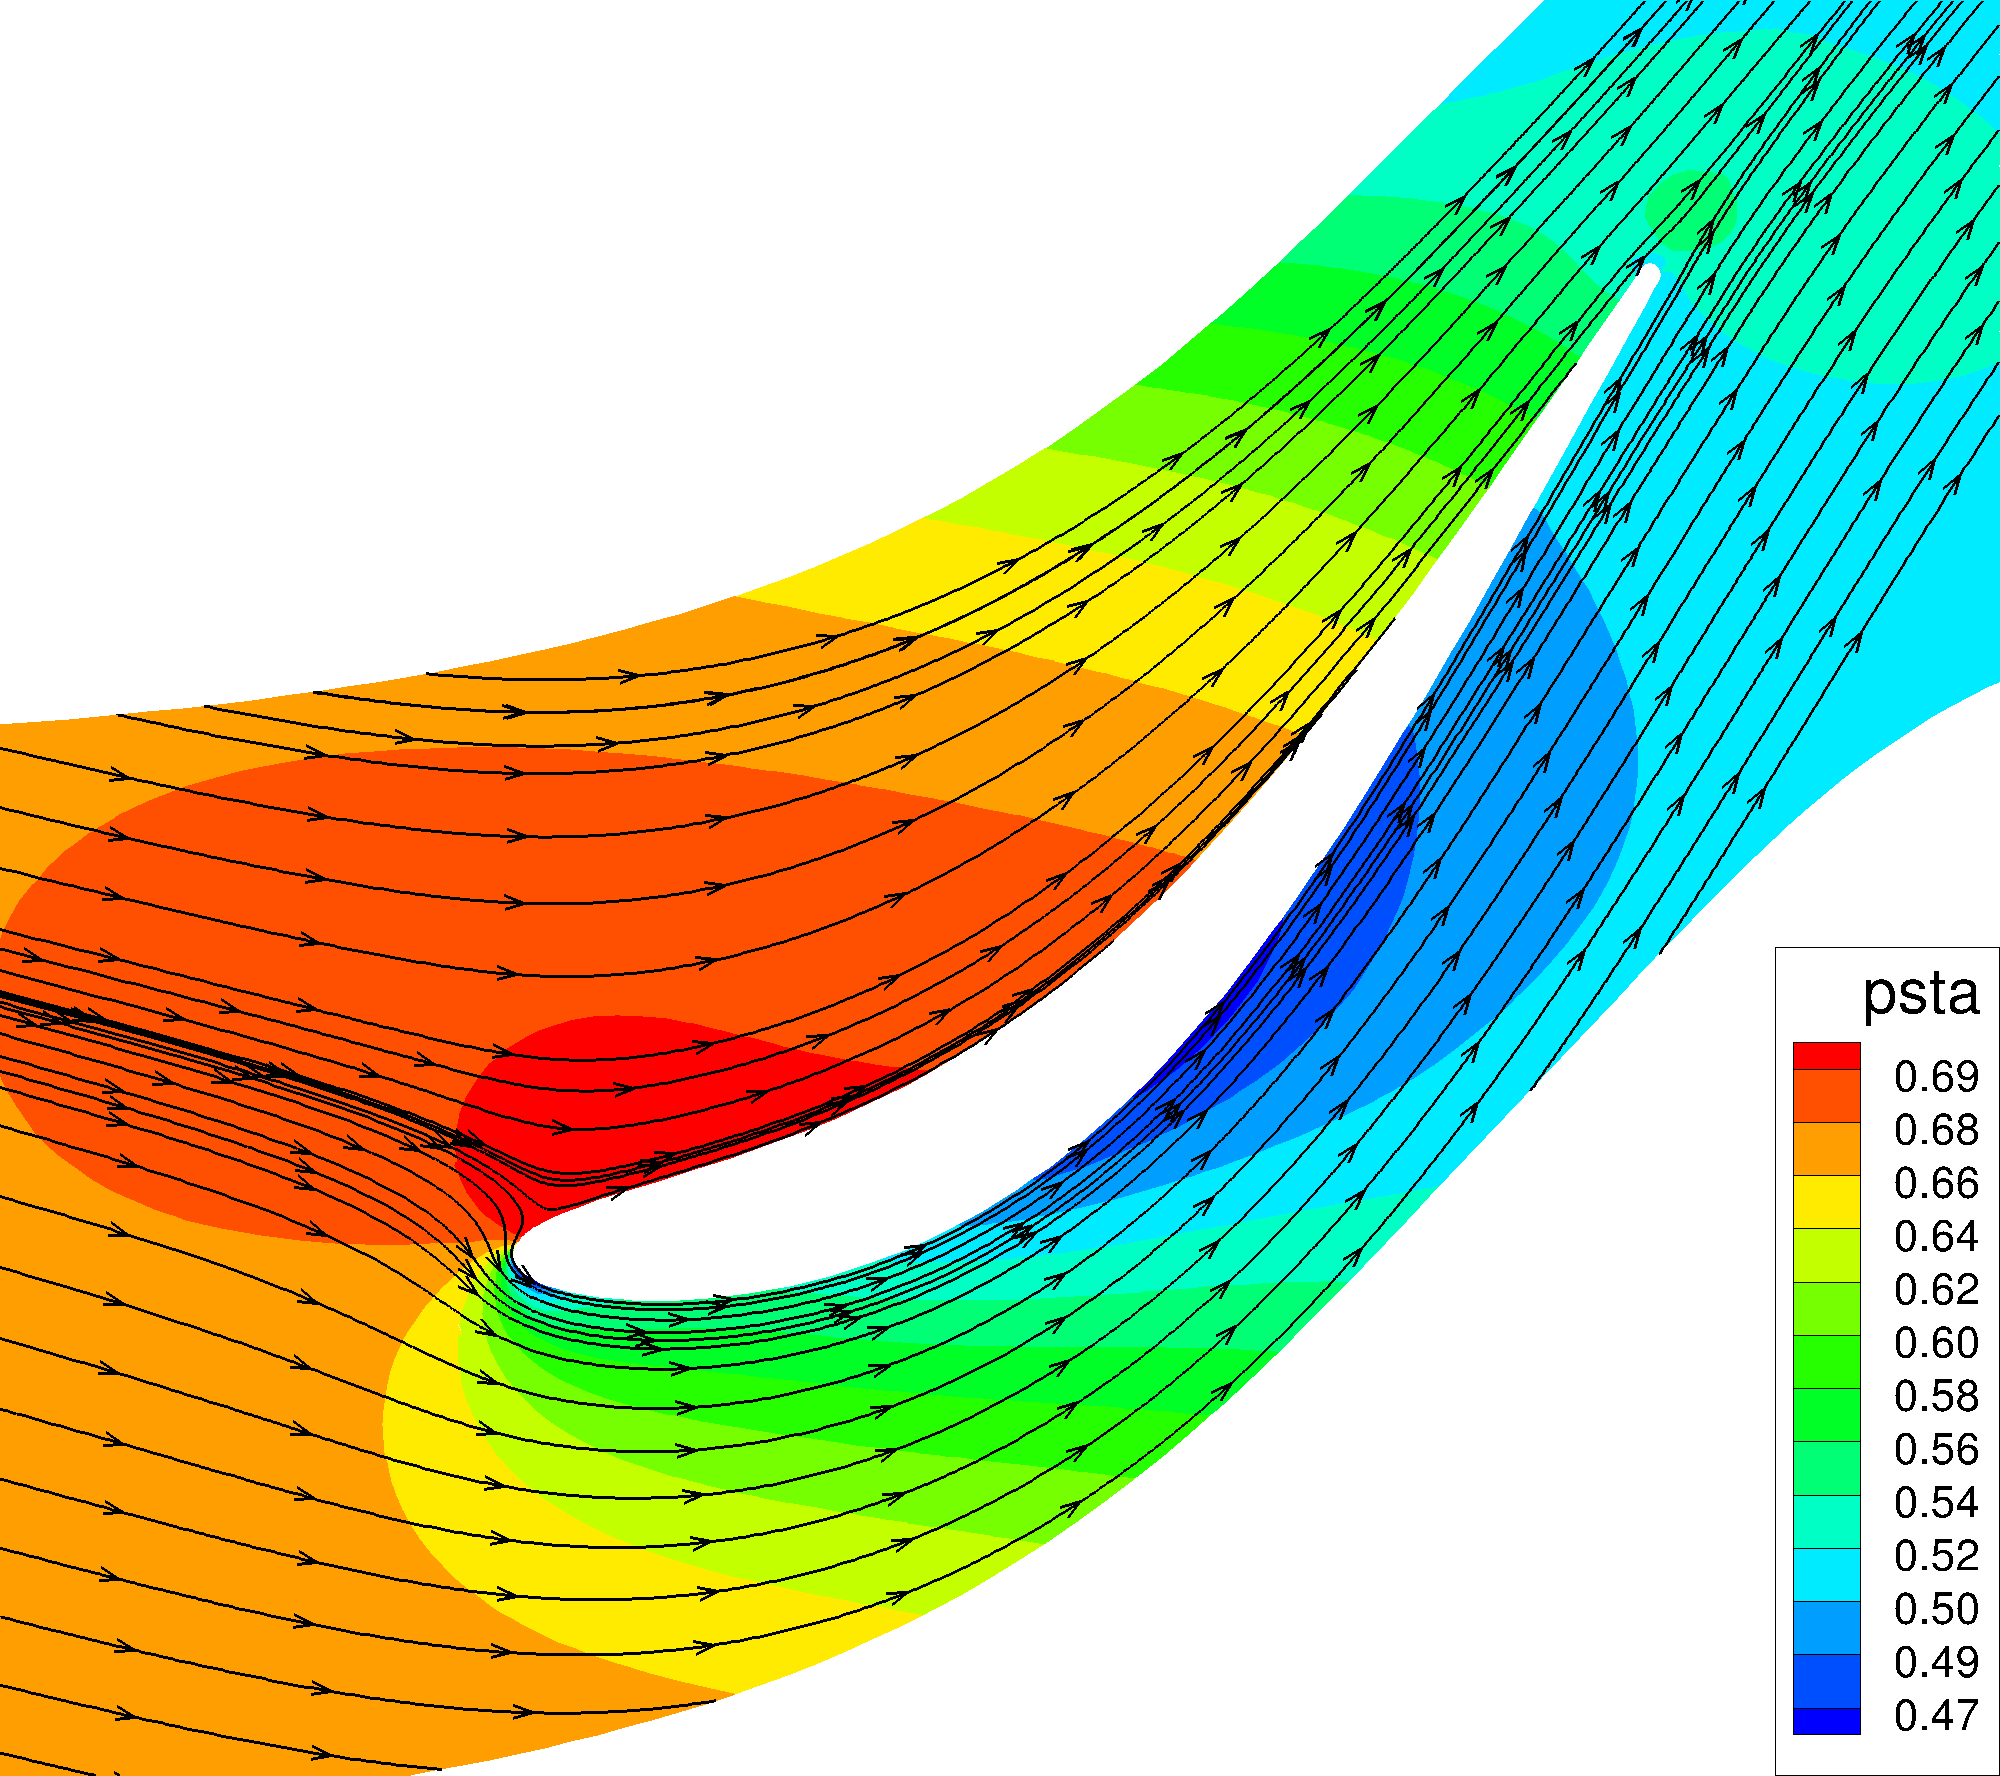
\includegraphics[height=.3\textwidth]{stcf11_subsonic_local.png}}
  \caption{Steady results for the STCF~11 configuration, subsonic case.}
  \label{fig:stcf11_rans_subsonic}
\end{figure}

\paragraph{Aeroelastic results}

% unsteady results
The aeroelastic experimental data are compared to the present results
obtained with both the DTS and the HB approach. To explore the range
of nodal diameters with the HB method, an incremental approach is used
where each nodal diameter simulation is used to initialize the next
one.  Considering the opposite phase vibration case (the 10\textsuperscript{th} nodal diameter), 
the amplitude and the phase of the pressure coefficient are
presented in Figure~\ref{fig:stcf11_ael_subsonic_ibpa_180_paper}.
With only one harmonic (\emph{i.e.} three instants), the HB results
are superimposed with the DTS ones. Moreover, the numerical results are
in fair agreement with the experimental data for the
amplitude. However, for the phase, the sign change on the
suction side is predicted at about $60~\%$ of the chord, whereas the
experimental location is about 25~\%.
\begin{figure}[htp]
  \centering
  \subfigure[amplitude]{
  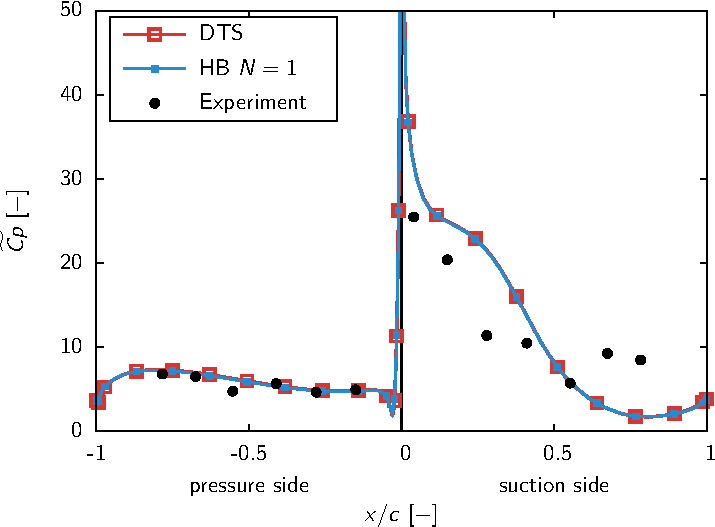
\includegraphics[width=.4\textwidth]{STCF11_AEL_SUBSONIC_IBPA_180_Cp_PPT.pdf}}
  \subfigure[phase]{
  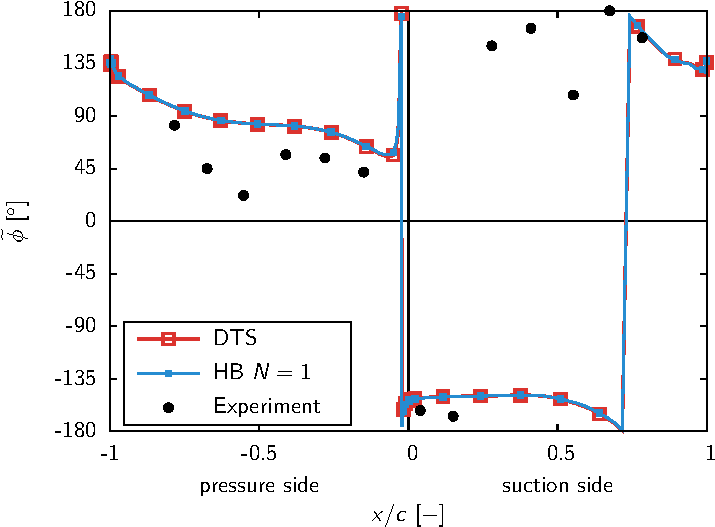
\includegraphics[width=.4\textwidth]{STCF11_AEL_SUBSONIC_IBPA_180_Phi_PPT.pdf}}
  \caption{Wall pressure harmonic analysis for an opposite phase vibration, subsonic case.}
  \label{fig:stcf11_ael_subsonic_ibpa_180_paper}
\end{figure}


The results for the  $-2$ nodal  diameter, corresponding to $\text{IBPA}=-36^\circ$, namely
the mostly damped as will be seen later on, are shown
in Figure~\ref{fig:stcf11_ael_subsonic_ibpa_324_paper}. The HB and DTS data
are superimposed, and are in fair agreement with the experiments. The
amplitude levels are well captured and the phase prediction is
slightly improved over the opposite phase case.
\begin{figure}[htp]
  \centering
  \subfigure[amplitude]{
  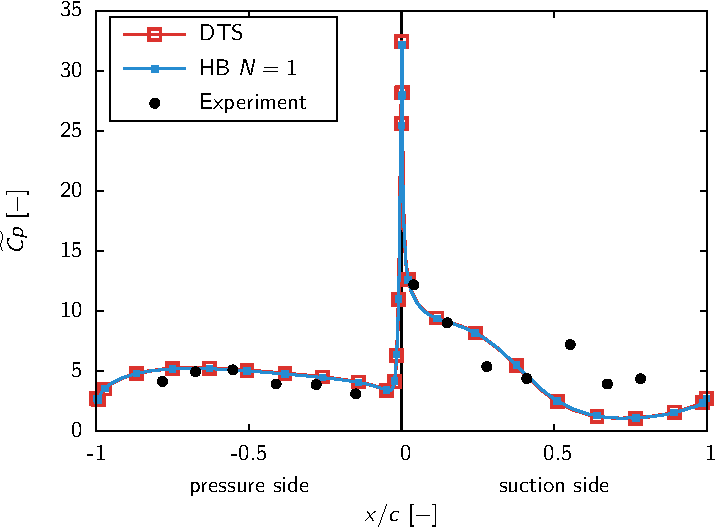
\includegraphics[width=.4\textwidth]{STCF11_AEL_SUBSONIC_IBPA_324_Cp_PPT.pdf}}
  \subfigure[phase]{
  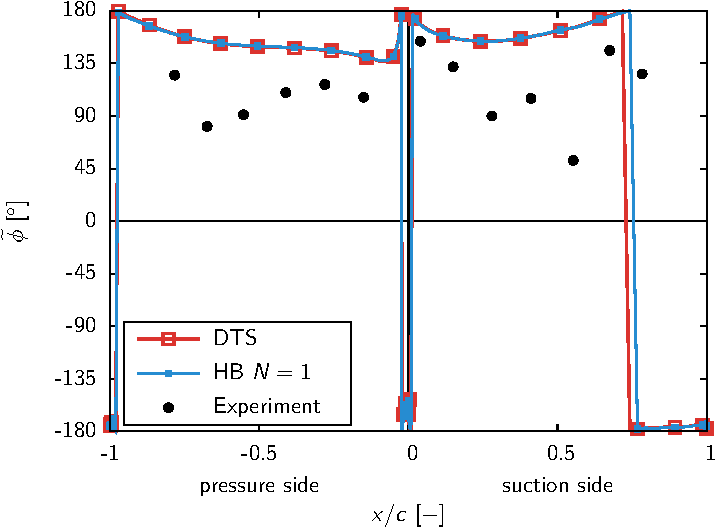
\includegraphics[width=.4\textwidth]{STCF11_AEL_SUBSONIC_IBPA_324_Phi_PPT.pdf}}
  \caption{Wall pressure harmonic analysis for a \mbox{$n_d=-2$}, subsonic case.}
  \label{fig:stcf11_ael_subsonic_ibpa_324_paper}
\end{figure}

The damping obtained from the previous calculations is depicted 
in Figure~\ref{fig:stcf11_subsonic_damping}.  Also plotted are the results
% from \citet{Fransson1999}, obtained with both
% potential, linear Euler, non-linear Euler and non-linear viscous codes.
from \citet{Fransson1999}, obtained with a
potential code.
% The results for all IBPAs are given for the potential code but only $\sigma=180^\circ$ is provided for the other codes~\cite{Fransson1999}.
These are the only damping results for the
subsonic case known by the authors.  Since the local variations are
superimposed for the DTS and the HB approaches, so are the damping.
The present
results show similar trends and levels to those of \citet{Fransson1999}.
\begin{figure}[htp]
  \centering
  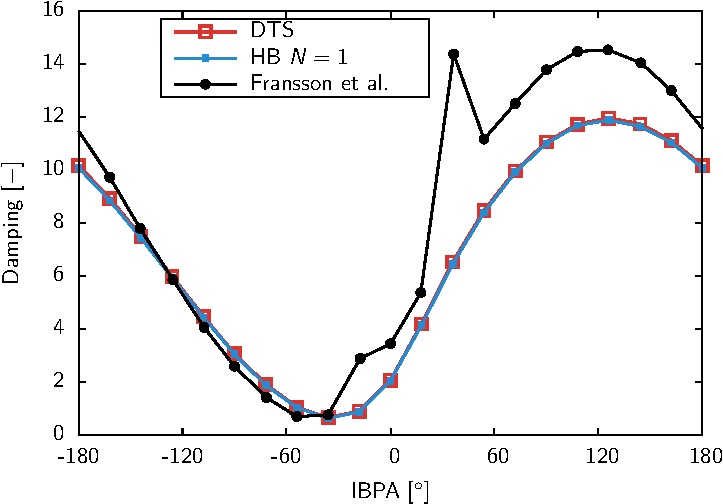
\includegraphics[width=.4\linewidth]{STCF11_SUBSONIC_DAMPING_PPT.pdf}
  \caption{Aerodynamic damping coefficient versus IBPA, subsonic case.}
  \label{fig:stcf11_subsonic_damping}
\end{figure}